\documentclass[a4paper]{article}
\usepackage[english]{babel}
\usepackage[utf8]{inputenc}
\usepackage[margin=1.15in]{geometry}
\usepackage{amsmath}
\usepackage{setspace}
\usepackage[colorinlistoftodos]{todonotes}
\usepackage{verbatim}
\usepackage{graphicx}
\usepackage[export]{adjustbox}
\usepackage{caption}
\setlength{\parskip}{\baselineskip}
\setlength{\parindent}{0pt}

\usepackage{enumitem}

\title{QF603 Group Mini-Project 3}

\author{Group F}

\date{\today}

\begin{document}
	\maketitle
	
	\begin{abstract}
	\vspace{6pt}
		In this report we performed 2 OLS regressions to understand the explanatory power of a number of factors - specifically those proposed by the CAPM and the Fama-French 5-Factor model. We observed that the factor with the most explanatory power is the market risk premium (Mkt-RF), as it has the largest t-test statistic. Overall, both models have high explanatory power as their adjusted $R^2$s are very close to 1.0. However, the 5-Factor model is deemed to be slightly better than the CAPM model.
	\end{abstract}

\newpage
\setcounter{secnumdepth}{1}
\section*{Task 5: OLS Regression}
\label{sec:introduction}

\subsection{Regression Estimation}
\setstretch{1.4}
\underline{CAPM}
\begin{itemize}[nosep]
	\item Y-Axis Intercept: $\hat{a}= -0.001710$
	\item Mkt-Rf Coefficient: $\hat{b}=0.964662$
\end{itemize}

\begin{figure}[ht]
	\centering
	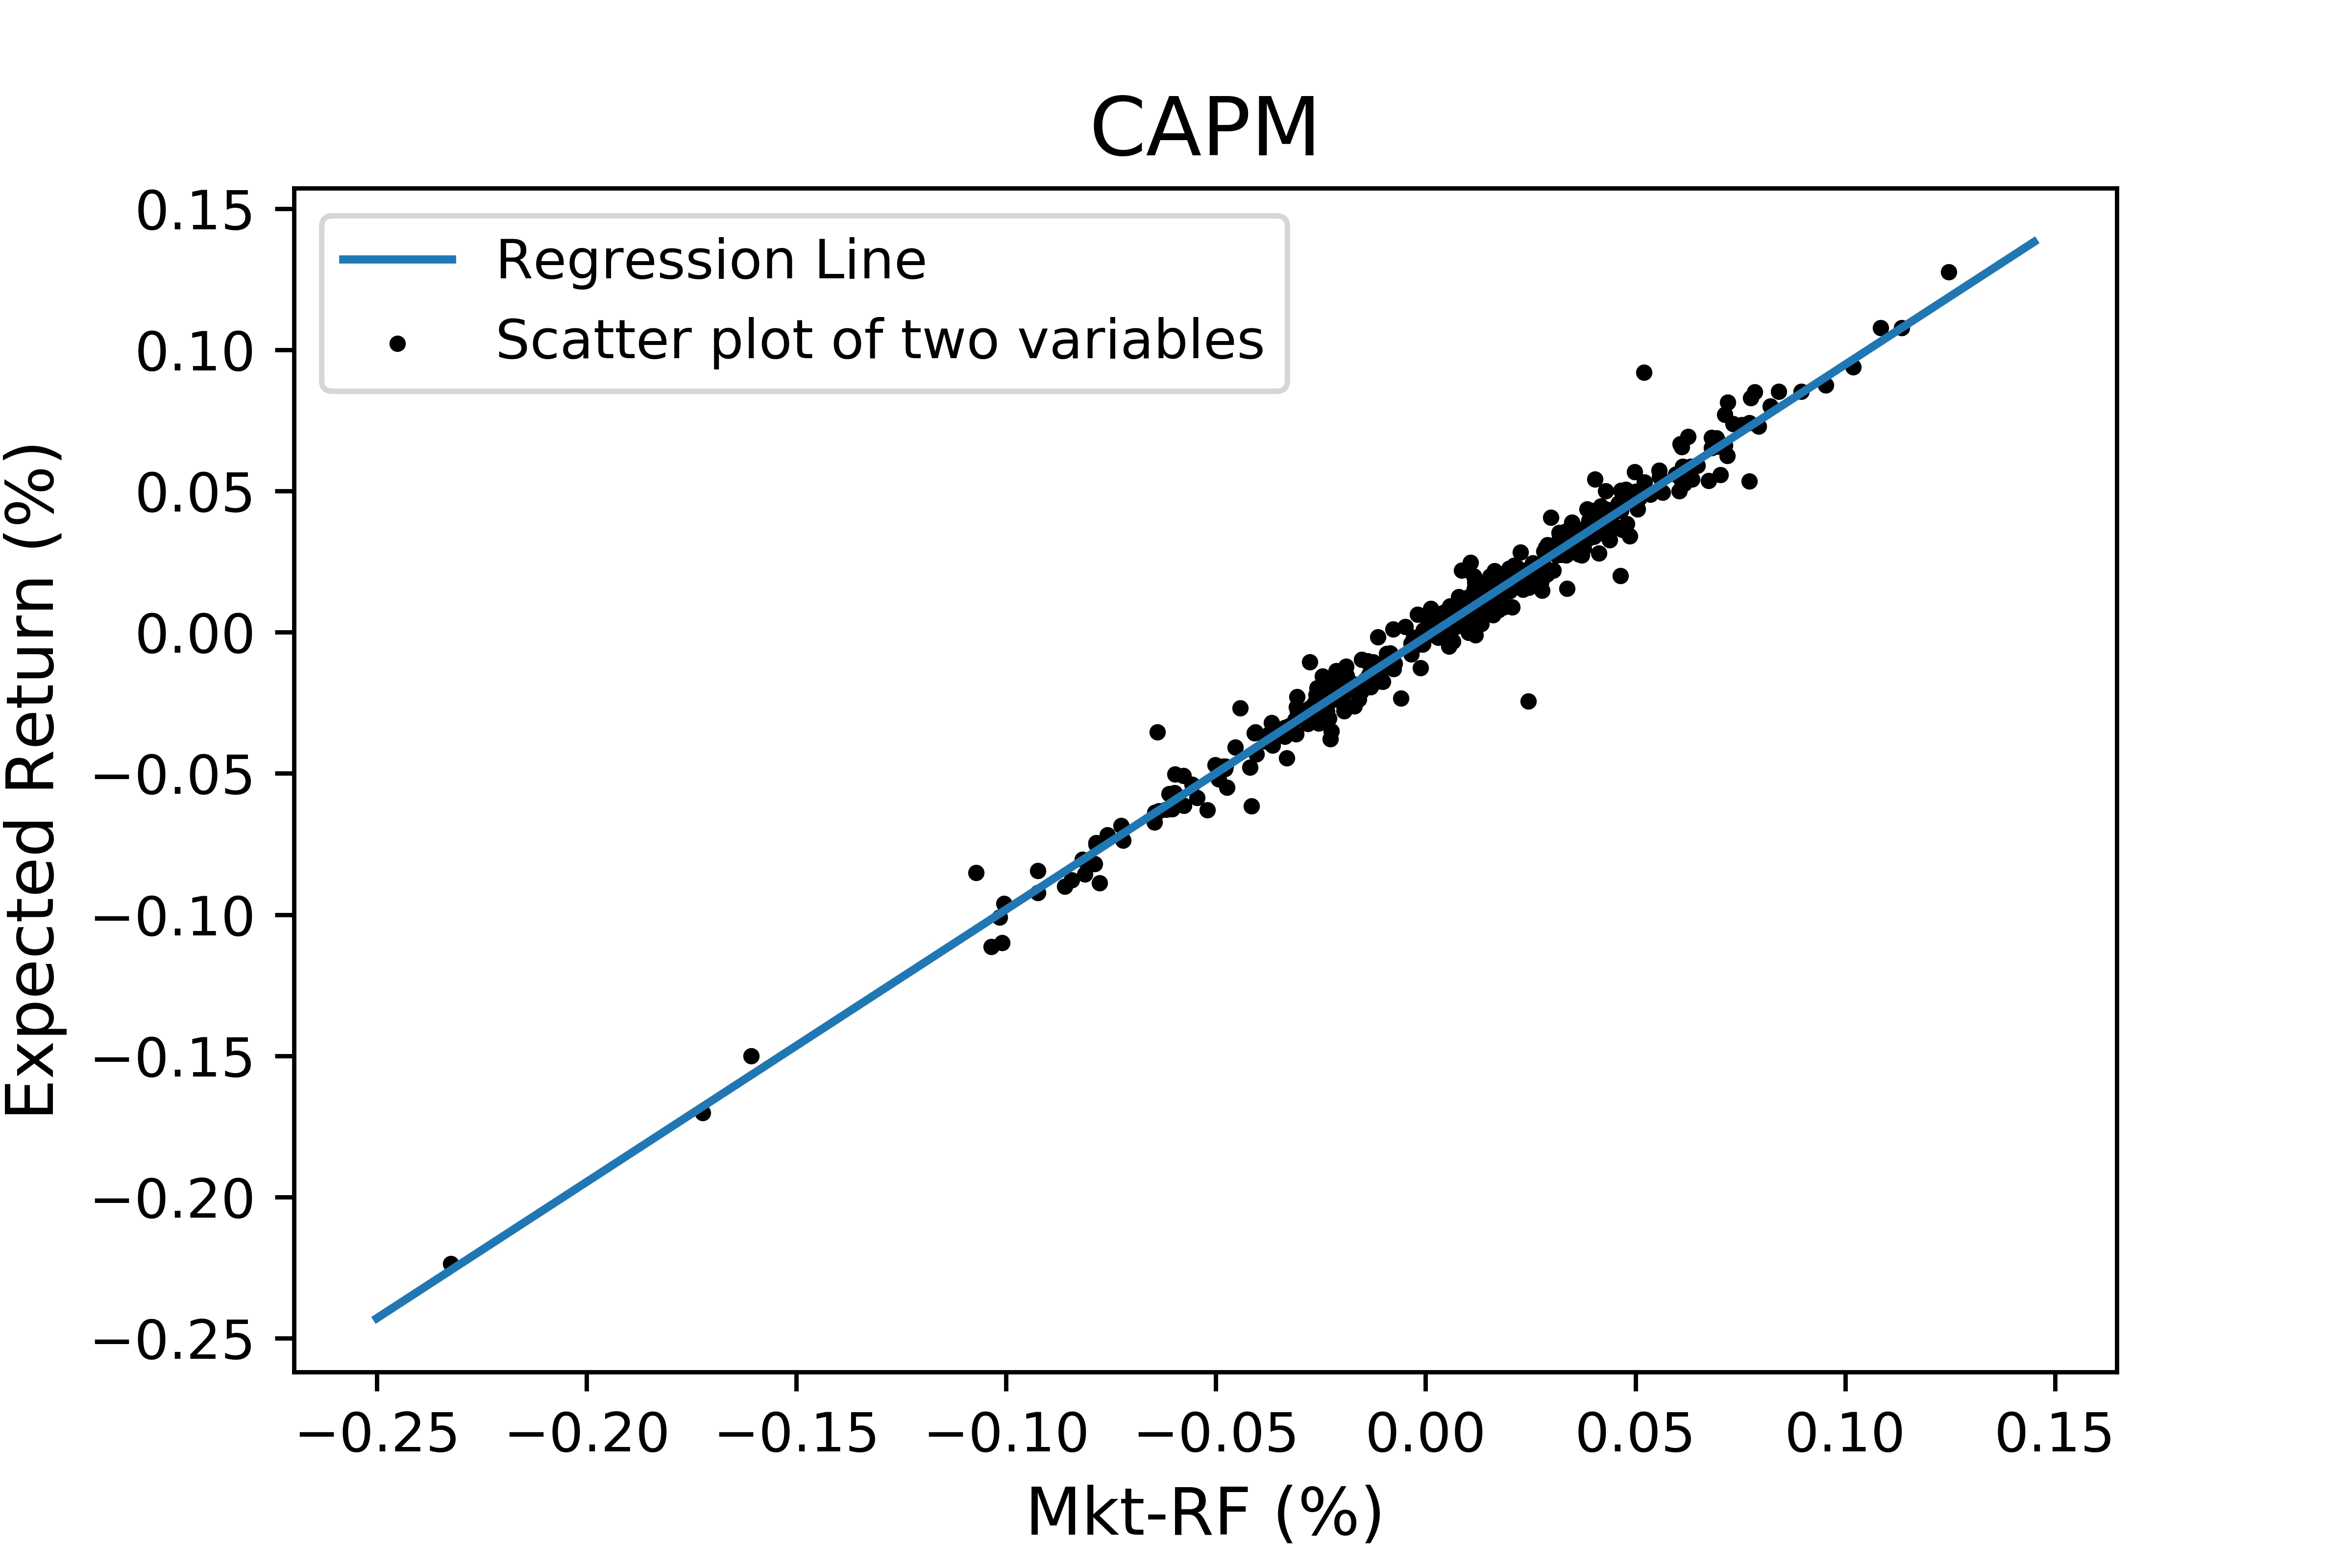
\includegraphics[width= \linewidth]{CAPM_regression.jpeg}
	\captionsetup{font=small}
	\caption{CAPM Regression Line}
\end{figure}

\underline{5-Factor Model}
\begin{itemize}[nosep]
	\item Y-Axis Intercept: $\hat{a} = -0.002257$
	\item Mkt-RF Coefficient: $\hat{b} = 1.009014$
	\item SMB Coefficient: $\hat{c} = -0.164592$
	\item HML Coefficient: $\hat{d} = 0.025487$
	\item RMW Coefficient: $\hat{e} = 0.059763$
	\item CMA Coefficient: $\hat{f} = 0.043634$
\end{itemize}

\newpage
\begin{figure}[ht]
	\centering
	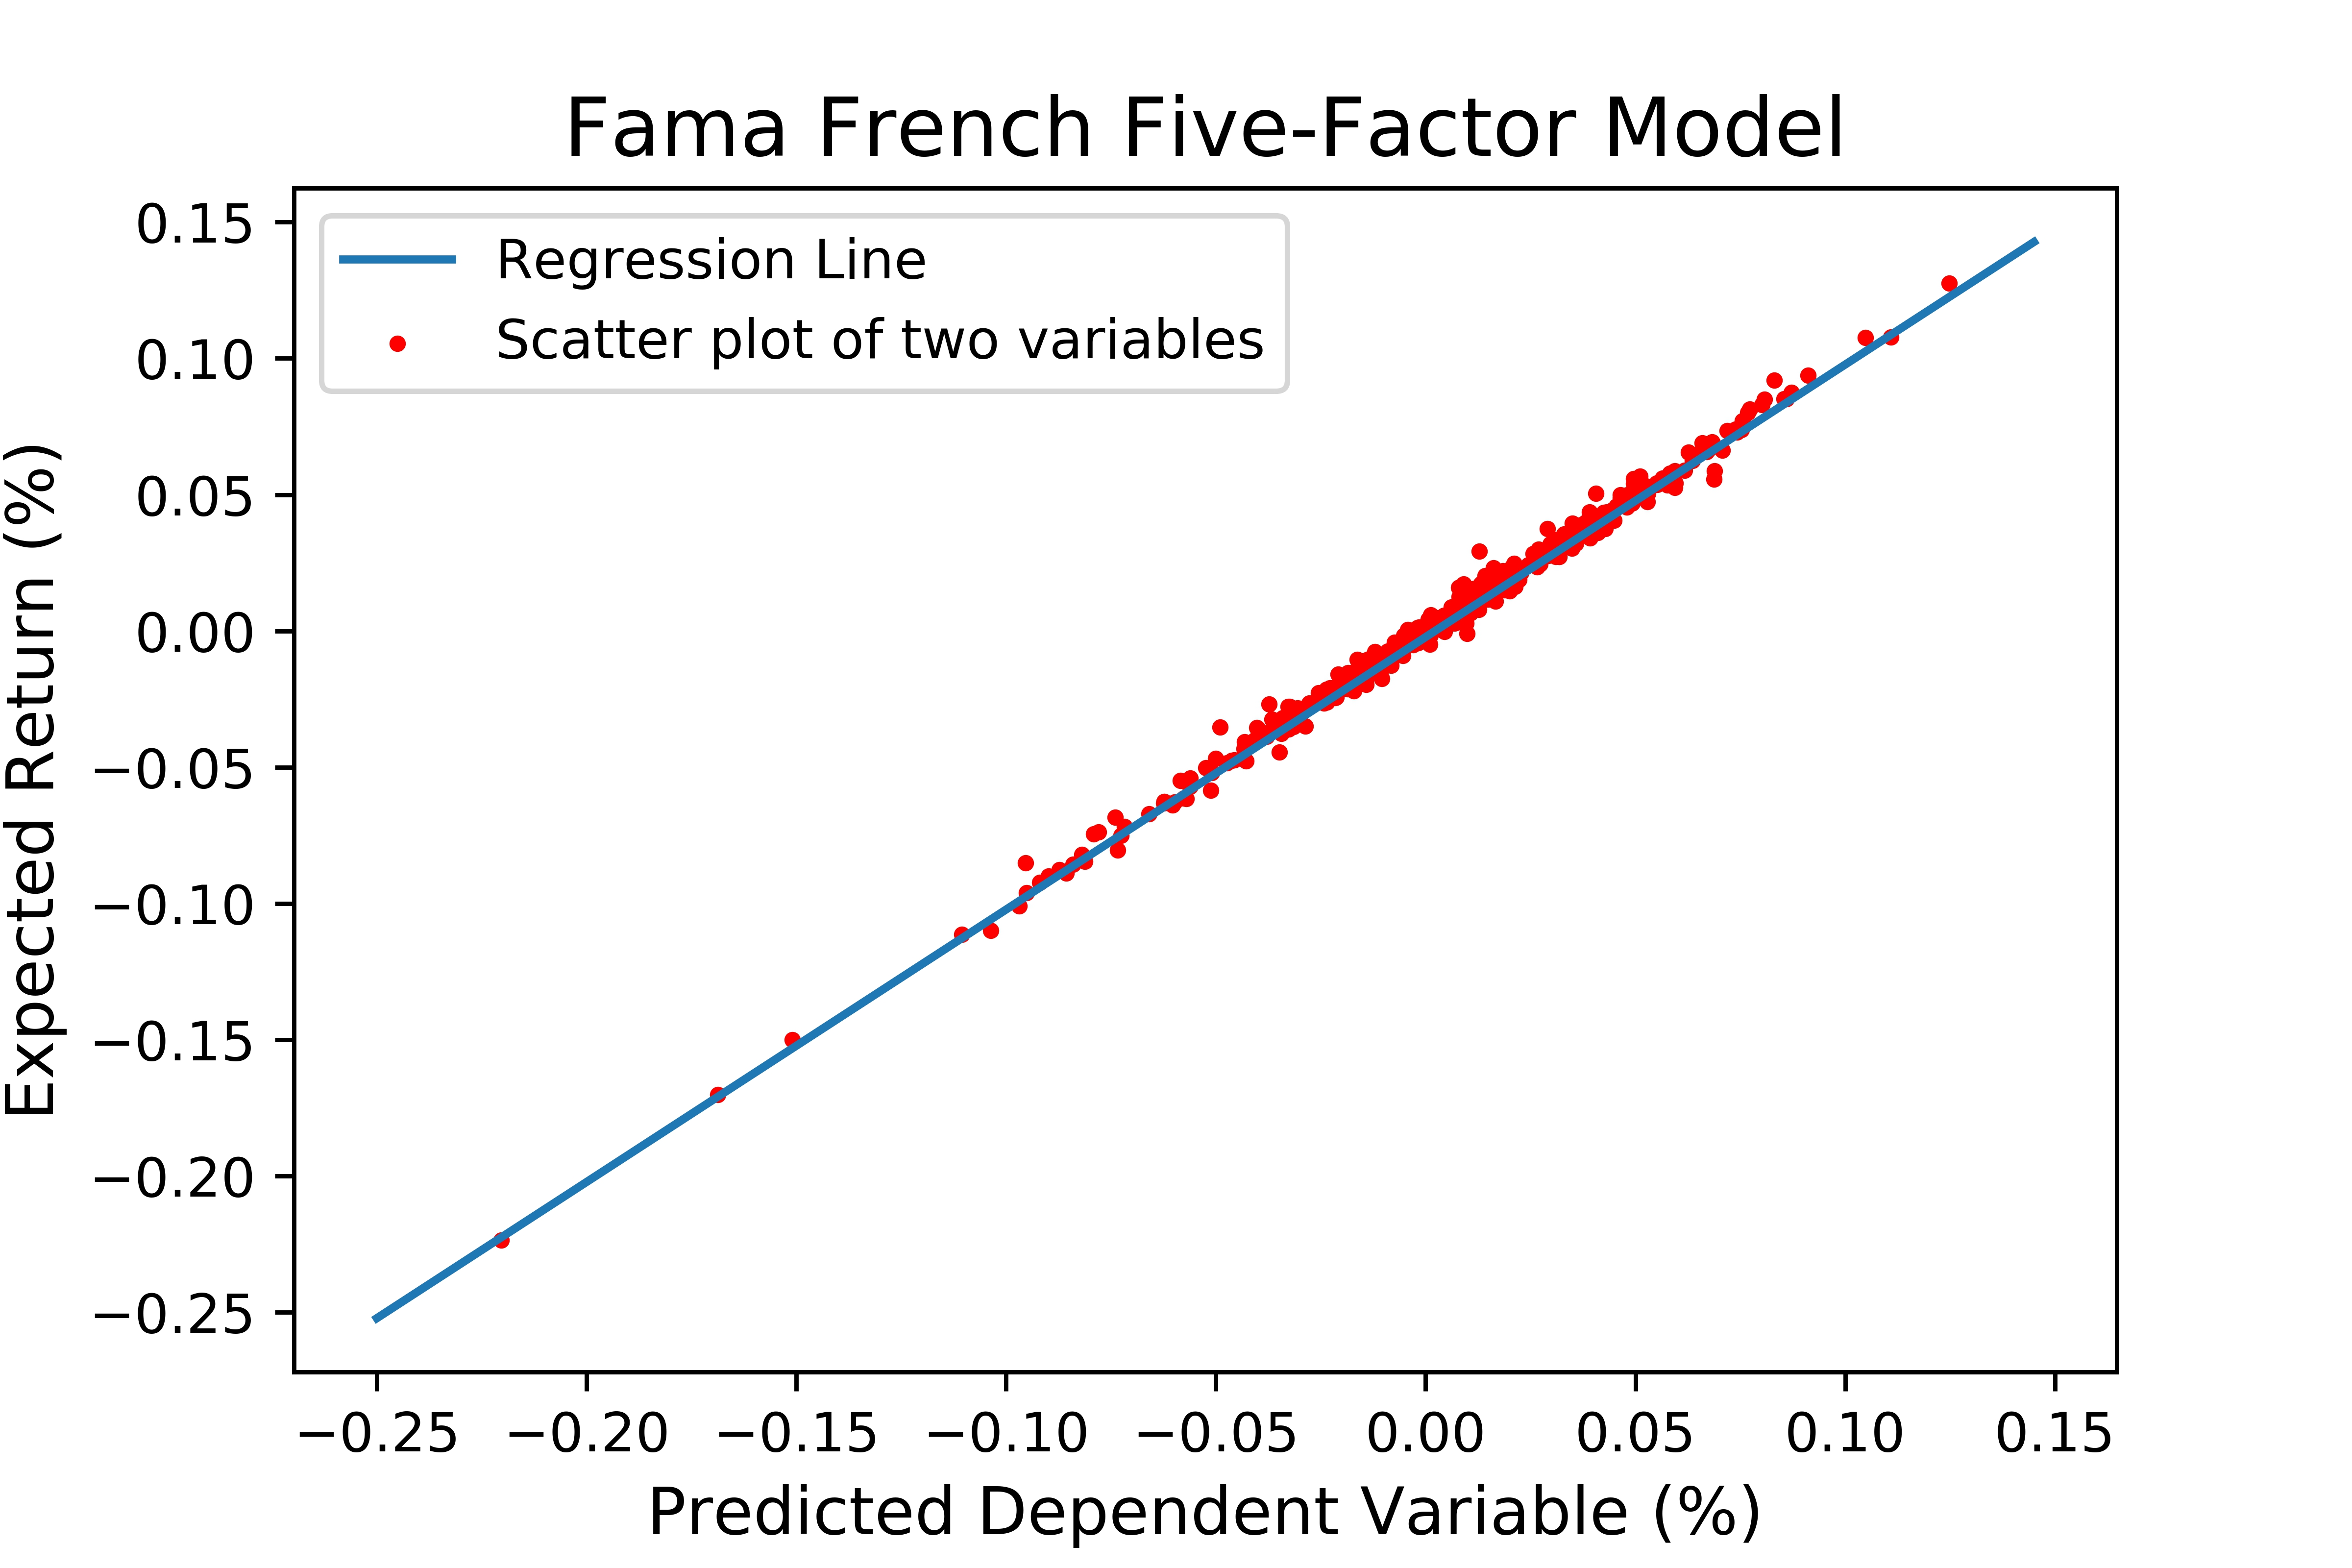
\includegraphics[width= \linewidth]{FF_regression.jpeg}
	\captionsetup{font=small}
	\caption{Five Factor Regression Line}
\end{figure}

\underline{Explanation}

Even after we added four more explanatory variables in the regression model, $\hat{b}$ the coefficient for the Mkt-RF explanatory variable and a measure of systematic risk, affects the dependent variable the most per unit change of the explanatory variable. 

$\hat{b}$ is greater than all the other coefficients combined, in absolute terms. The big correspondence between the returns of the market and the S\&P 500 shows why the S\&P 500 has often been used as a proxy for the U.S. equity market so far.

We also noted that the regression coefficient for the SMB (Small Minus Big) explanatory variable, $\hat{c}$, is negative and statistically different from 0 (see the t-test results in the next part). This makes intuitive sense as the S\&P 500 is made up of large cap companies, and as such should have its excess returns “penalised” to adjust for the “size effect” on returns. The “size effect”, also known as the “small firm” effect, is the proposition that smaller cap companies tend to outperform larger cap companies.

\newpage
\subsection{t-Test Results for Regression Coefficients}
\underline{Results for t-test}
\begin{itemize}
	\item t-Statistics for $\hat{a}$ = -12.890080, $\hat{b}$ = 230.124720, $\hat{c}$ = -26.268054, $\hat{d}$ = 3.172053, $\hat{e}$ = 7.213878, $\hat{f}$ = 3.720250
	\item Degrees of Freedom = 404 – 6 = 398
	\item Null Hypotheses ($H_0$) are that a = 0, b=0, c=0, d=0, d=0, e=0 and f=0
	\item Alternative Hypotheses ($H_1$) are that a$\ne$0 , b$\ne$0, c$\ne$0, d$\ne$0, e$\ne$0 and f$\ne$0
	\item Critical Values at 5\% Significance Level = $\pm$ 1.96594
	\item Critical Values at 1\% Significance Level = $\pm$ 2.58824
\end{itemize}

\underline{Explanation}

The t-test statistics for every regression coefficient fall outside of the $H_0$ acceptance range at the 5\% and even the 1\% levels of significance, and thus we reject the null hypotheses for all the coefficients that each of them has a value of zero.

We also note that the t-statistic for the $\hat{b}$ coefficient is extremely high and is as such extremely statistically significant. This also likely implies the comparatively outsized influence the Mkt-RF factor has on the S\&P 500’s excess returns when compared to the other four factors in the model.

We also conclude with a high level of confidence that linear relationships exist between the excess returns of the S\&P 500 index and each of Fama-French’s five factors – Mkt-Rf, SMB, HML, RMW, and CMA. 

\newpage
\subsection{$R^2$ and Adjusted $R^2$}
\underline{Results}
\begin{itemize}
	\item 5-Factor $R^2$=0.993902
	\item 5-Factor Adjusted $R^2$=0.993826
	\item CAPM $R^2$=0.975404
	\item CAPM Adjusted $R^2$=0.975343
\end{itemize}

\underline{Explanation}

Both and adjusted $R^2$ values are extremely close to 1, which implies that the Fama-French 5-Factor model is able to very well explain the monthly simple excess returns of the S\&P 500 index. 
We also found that the regression’s adjusted $R^2$ is only very slightly lower than its $R^2$. This suggests that the required downward adjustment to the model’s explanatory power to account for the loss of degrees of freedom associated with the model’s additional variables is very minimal. 
Furthermore, we found that the adjusted $R^2$ of the Fama-French 5-Factor model (0.993826) is slightly higher than the adjusted $R^2$ of the CAPM model (0.975343). While this suggests that the Fama-French 5-Factor model may slightly better explain the S\&P 500’s excess returns, it also highlights the possibility that Fama-French’s additional four factors (apart from market risk premium) may only provide marginal additional explanation of the S\&P 500’s excess returns. 

\subsection{Akaike Information Criterion (AIC)}
\underline{Results}
\begin{itemize}
	\item 5-Factor AIC = -4605.61
	\item CAPM AIC = -4050.15
\end{itemize}

\underline{Explanation}

Touching on measures of information, we found the AIC of the Fama-French 5-Factor model to be negative at -4605.61 and smaller than the CAPM’s AIC at -4050.15. The Fama-French 5-Factor model’s relatively smaller AIC suggests that it may be a better-quality model than the CAPM for estimating the S\&P 500’s excess returns. 

\newpage
\setcounter{secnumdepth}{1}
\section*{Task 6: F-Test Statistic}
\label{sec:introduction}

\begin{itemize}
	\item F-Test Statistic = 301.85
	\item Null Hypothesis $(H_0)$: $\hat{c}$ = 0, $\hat{d}$ = 0, $\hat{e}$ = 0, $\hat{f}$ = 0
	\item Alternative Hypothesis ($H_1$): $\hat{c}\ne$ 0, $\hat{d}\ne$ 0, $\hat{e} \ne$ 0, $\hat{f}\ne$ 0
	\item Critical Value at 5\% Significance Level = 2.394362
	\item Critical Value at 1\% Significance Level = 3.366592
\end{itemize}

\underline{Explanation}

The computed F-test statistic is extremely statistically significant at 301.85 and allows us to reject $H_0$ at both the 5\% and 1\% significance levels. From this, we are able to say with a high degree of confidence that the $\hat{c}, \hat{d}$, $\hat{e}$ and $\hat{f}$ coefficients are all not 0. 

This finding is similar to the ones we have made in Task 5, where we conducted t-tests to see if the individual regression coefficients are statistically different from zero.


\end{document}